\documentclass[letterpaper, 10 pt, conference]{ieeeconf} % Comment this line out if you need a4paper

% \documentclass[a4paper, 10pt, conference]{ieeeconf}   % Use this line for a4 paper

\overrideIEEEmargins                   % Needed to meet printer requirements.

% See the \addtolength command later in the file to balance the column lengths
% on the last page of the document

% The following packages can be found on http:\\www.ctan.org
\usepackage{graphicx} % for pdf, bitmapped graphics files
%\usepackage{epsfig} % for postscript graphics files
%\usepackage{mathptmx} % assumes new font selection scheme installed
%\usepackage{times} % assumes new font selection scheme installed
\usepackage{amsmath} % assumes amsmath package installed
\usepackage{amsfonts} % assumes amsmath package installed
\usepackage{amssymb} % assumes amsmath package installed

\title{\LARGE \bf
Meng Kiang SEAH, CID: 00699092
}

\author{EE4-54: Predictive Control. Assignment 5. % <-this % stops a space
}


\begin{document}

\maketitle
\thispagestyle{empty}
\pagestyle{empty}


%%%%%%%%%%%%%%%%%%%%%%%%%%%%%%%%%%%%%%%%%%%%%%%%%%%%%%%%%%%%%%%%%%%%%%%%%%%%%%%%
\begin{abstract}
Discussion of the results of Part A and B, and the conclusions drawn. Perhaps a little bit on the methods employed as well.
\end{abstract}


%%%%%%%%%%%%%%%%%%%%%%%%%%%%%%%%%%%%%%%%%%%%%%%%%%%%%%%%%%%%%%%%%%%%%%%%%%%%%%%%
\section{Part A - Tracking a Square}
The purpose of this part is to develop a controller that will move a cart around so that its suspended mass will track a square.

\subsection{Algorithm}
The method for tracking square revolves around how a square is defined. The simplest way is to describe it using the coordinates of its 4 corners. Thus, depending on the cart's location, it must move to the next corner as its target. The challenge with this is to determine how to change the cart's target with respect to its location.

The solution used in this case is to build a Simulink block that outputs the target depending on the current position of the cart. As the state variable contains the position of the cart, the Simulink block compares the $X$ and $Y$ values of the current state with the target state. Once the current state is sufficiently close to the target state (in terms of position as well as angle), the target state is changed to the following one.

To view the results, the positions of the cart and the mass were plotted, as will be seen in all the future figures. This helps to visualise the performance, and also helps to illustrate any interesting behaviour.

\subsection{Evaluation of Performance}\label{sec:error}
The method of evaluating the performance of the controller can be done by thinking of the ``perfect'' trajectory of the mass. This would be a square formed by the four coordinates. Looking down at the $XY$-plane, the area containing the path of the mass would be zero, as it would be made of 4 lines.

However, this is not going to be the case, as the movement of the cart will cause the mass to oscillate both in the $X$ and $Y$ directions. As such, the area containing the path would be non-zero. The calculation of this area can be done by looking at two rectangles. One is the smallest rectangle that contains the entire path. This is formed by looking at the maximum and minimum values of the $X$ and $Y$ values of the mass. The second rectangle is the largest rectangle that fits inside the path of the mass. This is calculated by looking at the largest deviation into the square as the mass moves along each segment of the square. The difference in area between the two squares is used as the error.

\subsection{Unconstrained Performance}
As mentioned, the purpose of a constraints in the controller is to improve the performance. Thus, that performance must be compared with the unconstrained version. Figure \ref{fig:rhc} shows the results. As mentioned, there is the path of the cart, the pendulum, and the corners, or the target states. Note also the circular margins around the corners. There are the margins around which the target state controller determines that the mass has reached the target state, and sets the target to the following state.

\begin{figure}[!ht]
    \centering
    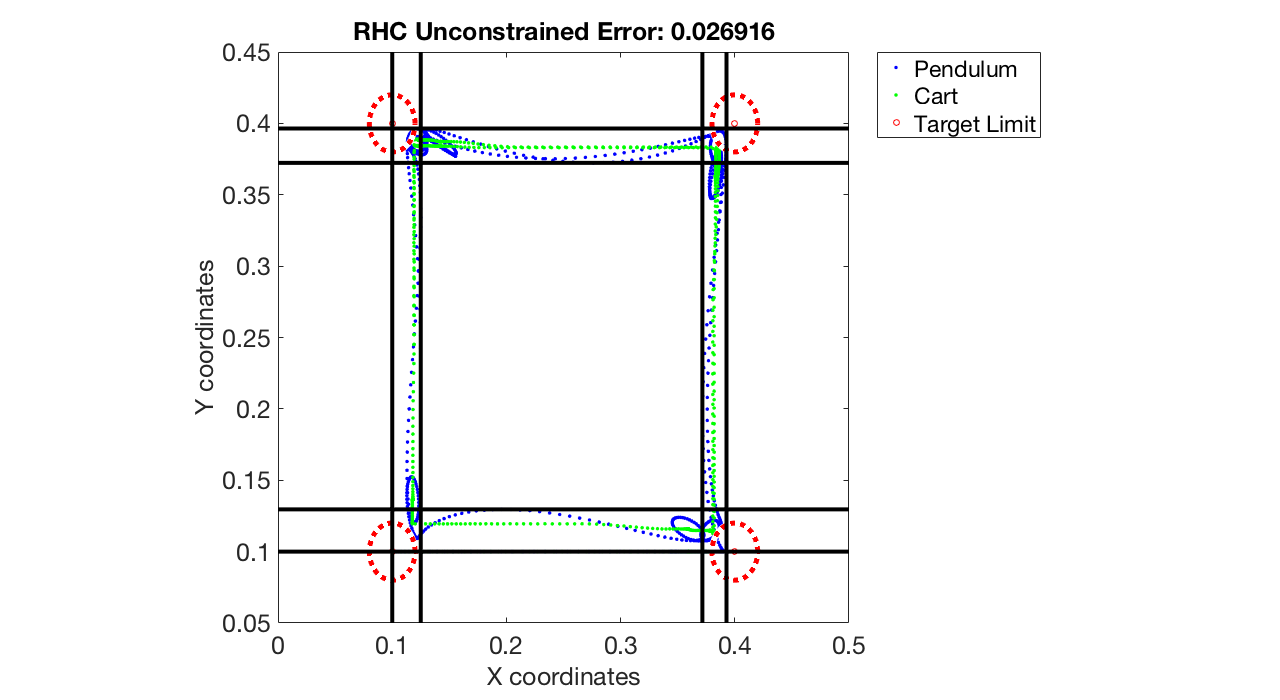
\includegraphics[width = 1.25\linewidth]{rhc}
    \caption{Path of the mass and cart with no constraints.}
    \label{fig:rhc}
\end{figure}

There are several observations. First is that the error as discussed in Section \ref{sec:error} is displayed in the title. Second, the limits of the two rectangles used to calculate this are shown with the black lines. As expected, the cart and mass do not move in a straight line. There is notably more disturbance around the corners, as the change of the direction of motion, combined with the laws of physics, mean that the mass does not make a perfect turn. It is safe to say that there is room for improvement.

\subsection{Constrained Performance}
Initially, the idea was to use the soft-constraints model from Assignment 4 for this section. However, discussions with others brought to light a paper from Frison and Jørgensen \cite{softconstraints}, describing the added computation complexity of the addition of soft-constraints. This was noticeable with just the basic codes from Assignment 4, where setting the sampling time as previously made a considerable increase in computation time. While this report does not include the hardware results, computation time is something to be mindful of. In fact, the linear simulation's time exceeded 15 seconds at peak (though this dwindled down).

Thus, the decision was made to run the controller with the hard constraints, and only to consider the soft constraints if the performance be poor enough to consider alternative methods. Again, the same target state calculator was used. The difference was that with the constraints, certain inputs to the MPC solver changed. This was because each target state affected the state constraints ($\hat{c}$, $\check{c}$), which went into the $\mathbf{b}$, and then into the $\mathbf{\tilde{b}}$ vector. Thus, another Simulink block was added, to choose from the 4 possible $\mathbf{\tilde{b}}$s. The 4 were precalculated to improve simulation time.

Only the non-linear simulation was used as the linear simulation failed to converge to a solution. 

The simulation output was graphed through the same method as previously, which yields Figure \ref{fig:mpc}.
\begin{figure}[!ht]
    \raggedleft
    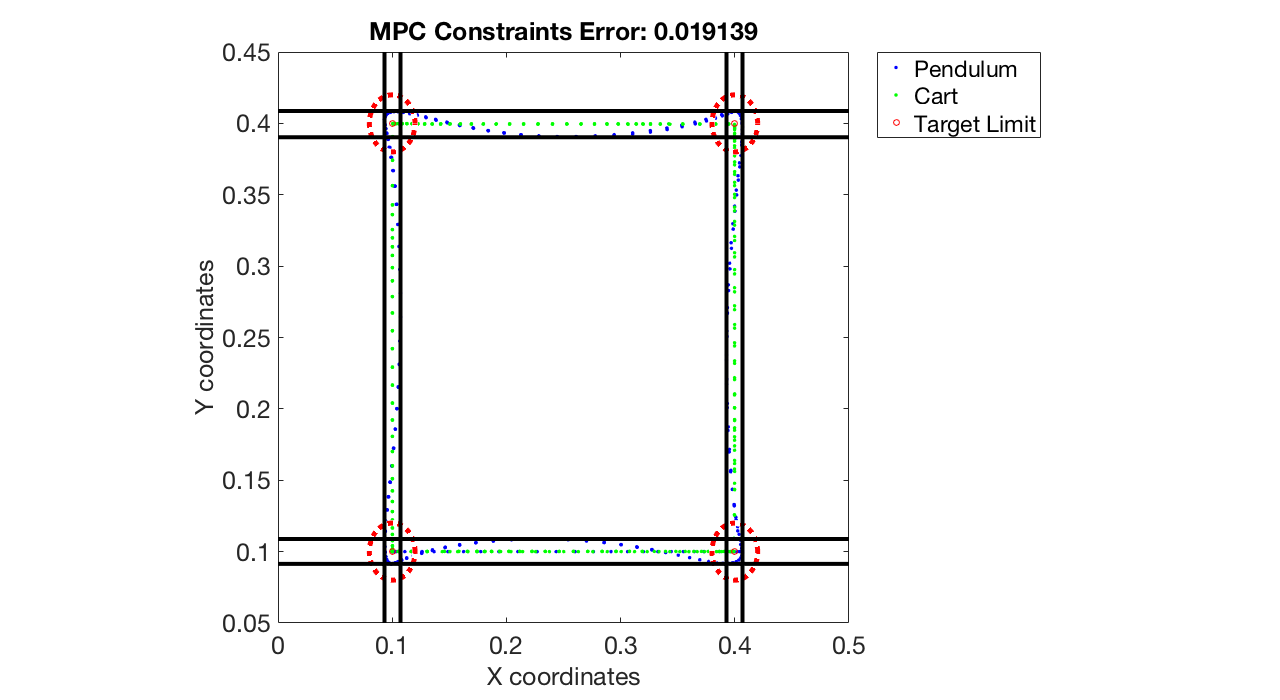
\includegraphics[width = 1.25\linewidth]{mpc}
    \caption{Path of the mass and cart with hard constraints.}
    \label{fig:mpc}
\end{figure}

Firstly, the error of 0.019139 from the MPC with hard constraints is much less than the error of 0.026916 from the unconstrained RHC. Thus, it makes sense to add constraints, as it may be more complex, but yields a better solution (as defined previously). Additionally, when looking at the acceptance margin of the corners of the square, the upper and lower limits of $X$ and $Y$ are found entirely contained. This method of solution judgement was not considered, but it shows how more precisely the controller executes its movements. The particular focus around the corners (where direction changing can be challenging) is intriguing as the points are the very definition of the path followed. Also to note is that the controller would cycle through the states if it had sufficient time and found a solution.

\subsection{Penalty Matrices}


\section{Part B - Q2: Tracking Non-Square Paths}


\begin{itemize}
    \item No
    \item Yes
\end{itemize}

\begin{align}
    J = \frac{1}{N} \sum_{n=1}^{N} \lvert \lvert x_n - \widetilde{x_n} \rvert \rvert ^2 = \sum_{i = M+1}^{D} \lambda_i \label{eq:erroreq}
\end{align}

Just a little check, Equation \ref{eq:erroreq}.

\subsection{Some Common Mistakes}
\begin{itemize}

    \item TA
    \item B
    \item Cy
    \item ID
    \item E
\end{itemize}

\subsection{Figures and Tables}
 \cite{IEEEexample:shellCTANpage} \cite{IEEEexample:IEEEwebsite}.

\begin{table}[h]
\caption{An Example of a Table}
\label{table_example}
\begin{center}
\begin{tabular}{|c||c|}
\hline
One & Two\\
\hline
Three & Four\\
\hline
\end{tabular}
\end{center}
\end{table}

\section{Conclusion}

A conclusion section is not required. Although a conclusion may review the main points of the paper, do not replicate the abstract as the conclusion. A conclusion might elaborate on the importance of the work or suggest applications and extensions.

\bibliographystyle{IEEEtran}
\bibliography{final}

% \addtolength{\textheight}{-12cm}  % This command serves to balance the column lengths
                 % on the last page of the document manually. It shortens
                 % the textheight of the last page by a suitable amount.
                 % This command does not take effect until the next page
                 % so it should come on the page before the last. Make
                 % sure that you do not shorten the textheight too much.

%%%%%%%%%%%%%%%%%%%%%%%%%%%%%%%%%%%%%%%%%%%%%%%%%%%%%%%%%%%%%%%%%%%%%%%%%%%%%%%%



\end{document}
